% questions.tex —— 2023 年·全国甲卷·理科 · 题目内容片段（无答案）
% 由 tools/generate_projects.py 依来源总账自 2023/2023_数学真题_全国甲理_试题.md 生成，勿手改（改源 MD 后重跑）


\par\medskip

\gkpart{一、单选题}

\begin{question}
\gkti{1}设全集 $U=\mathbb Z$，集合 $M=\{x\mid x=3k+1,\ k\in\mathbb Z\}$，$N=\{x\mid x=3k+2,\ k\in\mathbb Z\}$，则 $\complement_U(M\cup N)=$\mbox{（　　）}

\begin{gkopts}(2)
\task A．$\{x\mid x=3k,\ k\in\mathbb Z\}$
\task B．$\{x\mid x=3k-1,\ k\in\mathbb Z\}$
\task C．$\{x\mid x=3k-2,\ k\in\mathbb Z\}$
\task D．$\varnothing$
\end{gkopts}

\end{question}
\begin{question}
\gkti{2}设 $a\in\mathbb R$，$(a+\mathrm i)(1-a\mathrm i)=2$，则 $a=$\mbox{（　　）}

\begin{gkopts}(4)
\task A．$-2$
\task B．$-1$
\task C．$1$
\task D．$2$
\end{gkopts}

\Needspace{0.4\textheight}
\end{question}
\begin{question}
\gkti{3}执行如图的程序框图，则输出的 $B=$\mbox{（　　）}
\nopagebreak[4]
\begin{center}\begin{tikzpicture}[>=stealth, every node/.style={font=\small}]
  \node[draw, rounded corners, minimum width=1.15cm, minimum height=0.48cm] (start) at (0,7.2) {开始};

  \draw[->] (start.south) -- (0,6.78);
  \draw (-2.9,6.72) -- (2.9,6.72) -- (2.6,6.05) -- (-3.2,6.05) -- cycle;
  \node at (-0.15,6.38) {输入 $n=3,\ A=1,\ B=2,\ k=1$};
  \draw[->] (0,6.05) -- (0,5.52);

  \draw (-1.05,5.05) -- (0,5.5) -- (1.05,5.05) -- (0,4.6) -- cycle;
  \node at (0,5.05) {$k\leqslant n$};
  \node at (-0.18,4.36) {是};
  \node at (1.35,5.22) {否};

  \draw[->] (0,4.6) -- (0,4.13);
  \node[draw, minimum width=2.05cm, minimum height=0.5cm] (a) at (0,3.86) {$A=A+B$};
  \draw[->] (a.south) -- (0,3.36);
  \node[draw, minimum width=2.05cm, minimum height=0.5cm] (b) at (0,3.1) {$B=A+B$};
  \draw[->] (b.south) -- (0,2.6);
  \node[draw, minimum width=2.05cm, minimum height=0.5cm] (k) at (0,2.34) {$k=k+1$};
  \draw[->] (k.west) -- (-2.35,2.34) -- (-2.35,5.05) -- (-1.05,5.05);

  \draw[->] (1.05,5.05) -- (2.73,5.05) -- (2.73,1.16);
  \draw (2.05,1.12) -- (3.7,1.12) -- (3.42,0.55) -- (1.77,0.55) -- cycle;
  \node at (2.73,0.84) {输出 $B$};
  \draw[->] (2.73,0.55) -- (2.73,0.12);
  \node[draw, rounded corners, minimum width=1.15cm, minimum height=0.48cm] at (2.73,-0.18) {结束};
\end{tikzpicture}
\end{center}
\nopagebreak[4]
\begin{gkopts}(4)
\task A．$21$
\task B．$34$
\task C．$55$
\task D．$89$
\end{gkopts}

\end{question}
\begin{question}
\gkti{4}已知向量 $\boldsymbol a$，$\boldsymbol b$，$\boldsymbol c$ 满足 $|\boldsymbol a|=|\boldsymbol b|=1$，$|\boldsymbol c|=\sqrt2$，且 $\boldsymbol a+\boldsymbol b+\boldsymbol c=\boldsymbol0$，则 $\cos\langle\boldsymbol a-\boldsymbol c,\boldsymbol b-\boldsymbol c\rangle=$\mbox{（　　）}

\begin{gkopts}(4)
\task A．$-\dfrac45$
\task B．$-\dfrac25$
\task C．$\dfrac25$
\task D．$\dfrac45$
\end{gkopts}

\end{question}
\begin{question}
\gkti{5}设等比数列 $\{a_n\}$ 的各项均为正数，前 $n$ 项和为 $S_n$，若 $a_1=1$，$S_5=5S_3-4$，则 $S_4=$\mbox{（　　）}

\begin{gkopts}(4)
\task A．$\dfrac{15}{8}$
\task B．$\dfrac{65}{8}$
\task C．$15$
\task D．$40$
\end{gkopts}

\end{question}
\begin{question}
\gkti{6}某地的中学生中有 $60\%$ 的同学爱好滑冰，$50\%$ 的同学爱好滑雪，$70\%$ 的同学爱好滑冰或爱好滑雪。在该地的中学生中随机调查一位同学，若该同学爱好滑雪，则该同学也爱好滑冰的概率为\mbox{（　　）}

\begin{gkopts}(4)
\task A．$0.8$
\task B．$0.6$
\task C．$0.5$
\task D．$0.4$
\end{gkopts}

\end{question}
\begin{question}
\gkti{7}设甲：$\sin^2\alpha+\sin^2\beta=1$，乙：$\sin\alpha+\cos\beta=0$，则\mbox{（　　）}

\begin{gkopts}(2)
\task A．甲是乙的充分条件但不是必要条件
\task B．甲是乙的必要条件但不是充分条件
\task C．甲是乙的充要条件
\task D．甲既不是乙的充分条件也不是乙的必要条件
\end{gkopts}

\end{question}
\begin{question}
\gkti{8}已知双曲线 $C:\dfrac{x^2}{a^2}-\dfrac{y^2}{b^2}=1$（$a>0$，$b>0$）的离心率为 $\sqrt5$，$C$ 的一条渐近线与圆 $(x-2)^2+(y-3)^2=1$ 交于 $A$，$B$ 两点，则 $|AB|=$\mbox{（　　）}

\begin{gkopts}(2)
\task A．$\dfrac{\sqrt5}{5}$
\task B．$\dfrac{2\sqrt5}{5}$
\task C．$\dfrac{3\sqrt5}{5}$
\task D．$\dfrac{4\sqrt5}{5}$
\end{gkopts}

\end{question}
\begin{question}
\gkti{9}现有 $5$ 名志愿者报名参加公益活动，在某一星期的星期六、星期日两天，每天从这 $5$ 人中安排 $2$ 人参加公益活动，则恰有 $1$ 人在这两天都参加的不同安排方式共有\mbox{（　　）}

\begin{gkopts}(4)
\task A．$120$ 种
\task B．$60$ 种
\task C．$30$ 种
\task D．$20$ 种
\end{gkopts}

\end{question}
\begin{question}
\gkti{10}函数 $y=f(x)$ 的图象由函数 $y=\cos\left(2x+\dfrac\pi6\right)$ 的图象向左平移 $\dfrac\pi6$ 个单位长度得到，则 $y=f(x)$ 的图象与直线 $y=\dfrac12x-\dfrac12$ 的交点个数为\mbox{（　　）}

\begin{gkopts}(4)
\task A．$1$
\task B．$2$
\task C．$3$
\task D．$4$
\end{gkopts}

\end{question}
\begin{question}
\gkti{11}已知四棱锥 $P-ABCD$ 的底面是边长为 $4$ 的正方形，$PC=PD=3$，$\angle PCA=45^\circ$，则 $\triangle PBC$ 面积为\mbox{（　　）}

\begin{gkopts}(4)
\task A．$2\sqrt2$
\task B．$3\sqrt2$
\task C．$4\sqrt2$
\task D．$6\sqrt2$
\end{gkopts}

\end{question}
\begin{question}
\gkti{12}设 $O$ 为坐标原点，$F_1$，$F_2$ 为椭圆 $C:\dfrac{x^2}{9}+\dfrac{y^2}{6}=1$ 的两个焦点，点 $P$ 在 $C$ 上，$\cos\angle F_1PF_2=\dfrac35$，则 $|OP|=$\mbox{（　　）}

\begin{gkopts}(2)
\task A．$\dfrac{13}{5}$
\task B．$\dfrac{\sqrt{30}}2$
\task C．$\dfrac{14}{5}$
\task D．$\dfrac{\sqrt{35}}2$
\end{gkopts}

\par\medskip

\end{question}
\gkpart{二、填空题}

\begin{question}
\gkti{13}若 $f(x)=(x-1)^2+ax+\sin\left(x+\dfrac\pi2\right)$ 为偶函数，则 $a=$ \gkblank{}．

\end{question}
\begin{question}
\gkti{14}若 $x$，$y$ 满足约束条件

\nopagebreak[4]
\[
\begin{cases}
3x-2y\leqslant3,\\
-2x+3y\leqslant3,\\
x+y\geqslant1,
\end{cases}
\]

则 $z=3x+2y$ 的最大值为 \gkblank{}．

\end{question}
\begin{question}
\gkti{15}在正方体 $ABCD-A_1B_1C_1D_1$ 中，$E$，$F$ 分别为 $AB$，$C_1D_1$ 的中点。以 $EF$ 为直径的球的球面与该正方体的棱共有 \gkblank{} 个公共点。

\end{question}
\begin{question}
\gkti{16}在 $\triangle ABC$ 中，$\angle BAC=60^\circ$，$AB=2$，$BC=\sqrt6$，$\angle BAC$ 的角平分线交 $BC$ 于 $D$，则 $AD=$ \gkblank{}．

\par\medskip

\end{question}
\gkpart{三、解答题}

\begin{question}
\gkti{17}记 $S_n$ 为数列 $\{a_n\}$ 的前 $n$ 项和，已知 $a_2=1$，$2S_n=na_n$。

  (1) 求 $\{a_n\}$ 的通项公式；

  (2) 求数列 $\left\{\dfrac{a_{n+1}}{2^n}\right\}$ 的前 $n$ 项和 $T_n$。

\Needspace{0.4\textheight}
\end{question}
\begin{question}
\gkti{18}如图，在三棱柱 $ABC-A_1B_1C_1$ 中，$A_1C\perp$ 平面 $ABC$，$\angle ACB=90^\circ$，$AA_1=2$，$A_1$ 到平面 $BCC_1B_1$ 的距离为 $1$。
\nopagebreak[4]
\begin{center}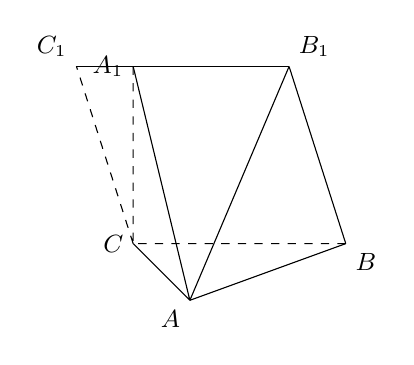
\begin{tikzpicture}[x=0.9cm,y=0.9cm,every node/.style={font=\small}]
  \coordinate (A)  at (1.8,0.2);
  \coordinate (B)  at (4,1);
  \coordinate (C)  at (1,1);
  \coordinate (A1) at (1,3.5);
  \coordinate (B1) at (3.2,3.5);
  \coordinate (C1) at (0.2,3.5);

  % 棱柱可见棱、遮挡棱，以及原图中标出的 A_1C 与 AB_1
  \draw (A)--(B) (A)--(C) (A)--(A1);
  \draw (A1)--(B1) (B1)--(C1) (C1)--(A1);
  \draw (B)--(B1) (A)--(B1);
  \draw[dashed] (B)--(C) (C)--(C1) (A1)--(C);

  \node[below left] at (A) {$A$};
  \node[below right] at (B) {$B$};
  \node[left] at (C) {$C$};
  \node[left] at (A1) {$A_1$};
  \node[above right] at (B1) {$B_1$};
  \node[above left] at (C1) {$C_1$};
\end{tikzpicture}
\end{center}
\nopagebreak[4]
  (1) 证明：$A_1C=AC$；

  (2) 已知 $AA_1$ 与 $BB_1$ 的距离为 $2$，求 $AB_1$ 与平面 $BCC_1B_1$ 所成角的正弦值。

\end{question}
\begin{question}
\gkti{19}一项试验旨在研究臭氧效应，试验方案如下：选 $40$ 只小白鼠，随机地将其中 $20$ 只分配到试验组，另外 $20$ 只分配到对照组，试验组的小白鼠饲养在高浓度臭氧环境，对照组的小白鼠饲养在正常环境，一段时间后统计每只小白鼠体重的增加量（单位：g）。

  (1) 设 $X$ 表示指定的两只小白鼠中分配到对照组的只数，求 $X$ 的分布列和数学期望；

  (2) 试验结果如下：

对照组的小白鼠体重的增加量从小到大排序为

$15.2\quad18.8\quad20.2\quad21.3\quad22.5\quad23.2\quad25.8\quad26.5\quad27.5\quad30.1$

$32.6\quad34.3\quad34.8\quad35.6\quad35.6\quad35.8\quad36.2\quad37.3\quad40.5\quad43.2$

试验组的小白鼠体重的增加量从小到大排序为

$7.8\quad9.2\quad11.4\quad12.4\quad13.2\quad15.5\quad16.5\quad18.0\quad18.8\quad19.2$

$19.8\quad20.2\quad21.6\quad22.8\quad23.6\quad23.9\quad25.1\quad28.2\quad32.3\quad36.5$

① 求 $40$ 只小白鼠体重的增加量的中位数 $m$，再分别统计两样本中小于 $m$ 与不小于 $m$ 的数据的个数，完成如下列联表：

\begin{center}
\begin{tabular}{ccc}
\toprule
 & $<m$ & $\geqslant m$ \\
\midrule
对照组 &  &  \\
试验组 &  &  \\
\bottomrule
\end{tabular}
\end{center}

② 根据①中的列联表，能否有 $95\%$ 的把握认为小白鼠在高浓度臭氧环境中与在正常环境中体重的增加量有差异？

\Needspace{10\baselineskip}
附：$K^2=\dfrac{n(ad-bc)^2}{(a+b)(c+d)(a+c)(b+d)}$，

\begin{center}
\begin{tabular}{cccc}
\toprule
$P(K^2\geqslant k)$ & $0.100$ & $0.050$ & $0.010$ \\
\midrule
$k$ & $2.706$ & $3.841$ & $6.635$ \\
\bottomrule
\end{tabular}
\end{center}

\end{question}
\begin{question}
\gkti{20}已知直线 $x-2y+1=0$ 与抛物线 $C:y^2=2px$（$p>0$）交于 $A$，$B$ 两点，$|AB|=4\sqrt{15}$。

  (1) 求 $p$；

  (2) 设 $F$ 为 $C$ 的焦点，$M$，$N$ 为 $C$ 上两点，且 $\overrightarrow{FM}\cdot\overrightarrow{FN}=0$，求 $\triangle MFN$ 面积的最小值。

\end{question}
\begin{question}
\gkti{21}已知函数 $f(x)=ax-\dfrac{\sin x}{\cos^3x}$，$x\in\left(0,\dfrac\pi2\right)$。

  (1) 当 $a=8$ 时，讨论 $f(x)$ 的单调性；

  (2) 若 $f(x)<\sin2x$，求 $a$ 的取值范围。

\end{question}
\begin{question}
\gkti{22}已知点 $P(2,1)$，直线 $l:\begin{cases}x=2+t\cos\alpha,\\y=1+t\sin\alpha,\end{cases}$（$t$ 为参数），$\alpha$ 为 $l$ 的倾斜角，$l$ 与 $x$ 轴正半轴、$y$ 轴正半轴分别交于点 $A$，$B$，且 $|PA|\cdot|PB|=4$。

  (1) 求 $\alpha$；

  (2) 以坐标原点为极点，$x$ 轴正半轴为极轴建立极坐标系，求 $l$ 的极坐标方程。

\end{question}
\begin{question}
\gkti{23}设 $a>0$，函数 $f(x)=2|x-a|-a$。

  (1) 求不等式 $f(x)<x$ 的解集；

  (2) 若曲线 $y=f(x)$ 与 $x$ 轴所围成的图形的面积为 $2$，求 $a$。

\end{question}